In this section, we present skyline computation algorithms. We first describe the concept of a pruning region, on which our algorithms are built. After foundations, two skyline algorithms are presented: Record-Based Pruning Skyline (RPS) is presented in Section~\ref{sec-RPS} and Index-Based Pruning Skyline (IPS) is presented in Section~\ref{sec-IPS}. Both RSP and IPS utilize the tree-based distributed index described in the previous section to build a set of pruning regions to eliminate unwanted data records. IPS generally provides better performance, but only produces correct result when the bounding boxes of the index tree does not overlap; whereas RSP works for any tree index.

The rest of this section describes pruning region. In the following definitions, when we say a point, $q$, and region, $R$, we mean a point and region in the data space such that ($q_1$, ..., $q_n$) are record attributes.

%In addition, to simplify our demonstration, we first consider 2-dimensional skyline. Later we show how our approach can be easily extended to higher dimensions.

%\begin{definition}[Pruning Region]
%Given the data space defined by $d_1 \times d_2 \times ... \times d_n$, where $d_i$ is the domain of attribute $i$, a pruning region is a pair of a pivot point and an ordered list of preference specifiers $(p, \sigma)$ that specifies a region of the data space that has been dominated by a subset of the data set. As defined in Section~\ref{sec-prelim}, $\sigma_i$ is one of the values in $\{min, max\}$.
%\end{definition}

\begin{definition}[Pruning Region]
A pruning region, $R$($d$, $\sigma$), is a rectangular region of data space that is dominated by one or more data records. $d$ is a point called dominant point and $\sigma$ is an ordered list of preference specifiers.
\end{definition}

Given an arbitrary point $d$ and $\sigma$, a pruning region $R$ is defined such that for each attribute $i$, if $\sigma_i = min$, then $d_i$ is the lower bound of $R$ for the $i$th dimension and the region extends to the maximal value for the $i$th dimension. Similarly, if $\sigma_i = max$, then $d_i$ is the upper bound and extends to minimal value of the dimension.

A dominant point can also be defined with any rectangle as follows:

\begin{definition}[Dominant Point]\label{def-dominant-point}
Given a n-dimensional rectangle, $B$, and a list of skyline preference specifiers, $\sigma$, the dominance point of the rectangle $d$($B$, $\sigma$) is the point of intersection of all axes of the data space and contains the ``best" of all axes in $B$, where the ``best" is defined by $\sigma$.
\end{definition}

The ideas of dominant point and pruning region are illustrated in Figures~\ref{fig:rtree_pr} where pruning regions are illustrated as the gray regions and dominant points are solid dots. The figure shows a 2-dimensional (Figure~\ref{fig:rtree_pr_2d}) and a 3-dimensional (Figure~\ref{fig:rtree_pr_3d}) data space with 2 pruning regions defined by dominant points $b$ and $d$. As illustrated, a pruning region is a region of an n-dimensional space that has been dominated by pivot point and can be ignored in the upcoming broadcast data stream.
By Definition~\ref{def-dominant-point}, we have the following properties:

\begin{property}\label{property:record_pruning}
Given $\sigma$, a pruning region can be constructed from any arbitrary data record, $p$, as $R$($p$, $\sigma$).
\end{property}

\begin{property}\label{property:pivot_point}
The dominant point of pruning region $R$ dominates all data points and minimal bounding rectangles inside $R$.
\end{property}

\begin{figure}[!h]
\centering
\subfigure[2-D space with $\sigma$ = ($min$, $min$).]{
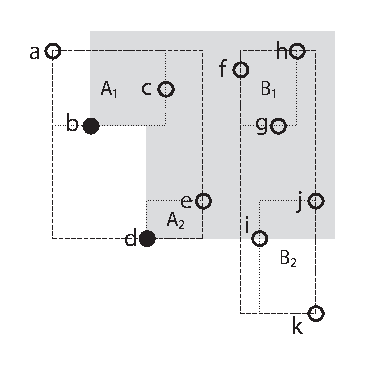
\includegraphics[width=1.5in]{Figures/rtree_pr2.eps}\label{fig:rtree_pr_2d}}
\subfigure[3-D space with $\sigma$ = ($min$, $min$, $max$).]{
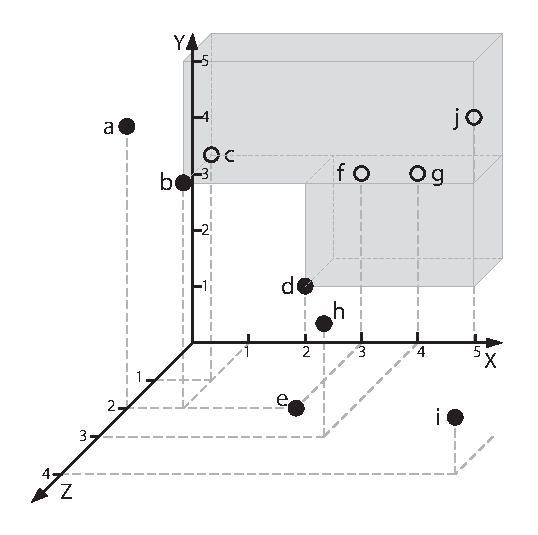
\includegraphics[width=1.5in]{Figures/rtree_pr_3d.eps}\label{fig:rtree_pr_3d}}
\caption{Pruning region with candidate Skyline points.\label{fig:rtree_pr}}
\end{figure}

Our skyline algorithms utilize pruning regions to determine if a record (a point in data space) or a branch of the index (a bounding rectangle) from the broadcast program can be ignored. The data items (record or index) that can be ignored are the ones that are covered by (or inside) any of the pruning regions that the skyline algorithm constructs and maintains. The following lemma determines if a data record covered by a pruning region.

\begin{lemma}\label{lemma:point_covered}
A data record, $p$, is covered by a pruning region $R$($d$, $\sigma$), if for each attribute $i$, one of the following is met:
\begin{enumerate}
  \item If $\sigma_i$ = $min$, then $p_i \geq d_i$
  \item If $\sigma_i$ = $max$, then $p_i \leq d_i$
\end{enumerate}
\end{lemma}

Lemma~\ref{lemma:point_covered} says to check if a data record, $p$, is covered by a pruning region, all attributes of the record has to be compare against the dominant point(or record), $d$, of the pruning region. If any attribute does not satisfy any of the two conditions, the record is not covered.

To determine if a branch of the broadcast index is covered by a pruning region, we need to compare the minimal bounding box of the index branching to the pruning region. By Property~\ref{property:pivot_point}, the following determines if a rectangle (bounding box) is covered.

\begin{lemma}\label{lemma:rect_covered}
Given a pruning region $R$($d$, $\sigma$) and a rectangle $B$, $R$($d$, $\sigma$) covers $B$ if $R$($d$, $\sigma$) covers the dominant point of $B$, $d$($B$, $\sigma$).
\end{lemma}

\begin{proof}
The pruning region $R$($d$, $\sigma$) covering the dominance point $d$($B$, $\sigma$) of $B$ implies that one of the conditions of Lemma~\ref{lemma:point_covered} is true for every attribute and that $d$ $\succ$ $d$($B$, $\sigma$). Due to Property~\ref{property:pivot_point}, $d$ $\succ$ $B$.
\end{proof}

An example is given in Figure~\ref{fig:pruning}. A pruning region $R$($s$, $\sigma$) is illustrated in gray with $\sigma$ = ($X$ = $min$, $Y$ = $max$). Bounding box $A$ can be pruned since its dominant point, $d$($A$, $\sigma$), falls inside the pruning region, while bounding box $B$ cannot be pruned since, although it is partially covered, its dominant point,  $d$($B$, $\sigma$), does not fall inside the pruning region.

\begin{figure}
\begin{center}

\includegraphics[width=2in]{Figures/pruning.eps}
\vspace*{-5pt} \caption{A pruning region defined by $d$ and
$\sigma$ = $(X = min, Y = max)$.} \vspace*{-5pt}
\label{fig:pruning}
\end{center}
\end{figure}



\subsection{Record-Based Skyline Pruning}\label{sec-RPS}

In this section, we present our skyline algorithm that utilizes the data records received from the broadcast program to construct pruning regions. At the beginning of the algorithm, the list of pruning regions, maintained by the algorithm, is empty. At this state, the algorithm cannot prune any broadcast item (index or data); therefore stays tuned into the channel and follows the index to the first data segment. As the algorithm receives data records, it constructs one pruning region for each data record as state in Property~\ref{property:record_pruning}. The following summarizes the notations we use in algorithm listings:

\begin{table}[!h]
\centering \caption{Algorithmic Notations}\label{tab:alg}
\begin{tabular}{|c|p{2in}|}
\hline
{\bf Symbol} & {\bf Description}\\
\hline\hline
$S$ & A set of candidate skylines; $S'$ denote local skylines.\\
$R$ & A set of pruning regions; $R'$ denotes local pruning region.\\
GetBucket($E$) & Wait and download items specified by $E$. \\
Skyline($B$, $\sigma$) & Compute skyline from set $B$ via NN. \\
GetPRegions($S$, $\sigma$) & Compute pruning regions from set $S$. \\
Prune($S$, $R$) & Remove items from $S$ that are covered by $R$.\\
\hline
\end{tabular}
\end{table}

The RPS algorithm is shown in Algorithm~\ref{alg:RBSkyline}. During initialization (line 1-2) of the algorithm, the list of candidate skylines, $S$, and the list of pruning regions, $R$, are assigned the empty set.

After initialization, the algorithm goes into the outer loop (line 3-32) that iterates through all branches of the index tree. For the first iteration, the first index bucket is downloaded (line 5-6). If the bucket is the root node of the index, then there is no sibling branch and $next$ remains $null$; otherwise, $next$ is set to the time of the next index segment(line 10-12), which contains the next branch.

In the inner loop (line 13-31), the algorithm pops the next data item, a bucket, to be downloaded, and downloads the data item (line 15). If the bucket downloaded is index, then each index entry, expressed as ($mbr$, $time$) pair, is push onto the stack (line 17-22). If bucket is not index, but is data, then the following are performed (line 23-30).

\begin{enumerate}
\item Computes local skyline, $S'$, of the data bucket (line 24).
\item Computes local pruning regions, $R'$, from $S'$ (line 24).
\item Prune records in $S$ and stack entries covered by $R'$ (line 26-27).
\item Add (union) local pruning regions, $R'$, to global regions, $R$ (line 28).
\item Add (union) local skyline,$S'$, to global skyline, $S$ (line 29).
\end{enumerate}

Note that $S$ are candidate skyline since there could be data objects broadcast later that dominate the earlier candidate Skyline points. For example, if a later candidate point $s'$ dominates an earlier point $s$, then $s$ is removed from $S$ and the pruning region is enlarged by the later point $s'$.

The skyline computation phase ends when the stack is empty and $S$ is returned as skyline (line 33).

\begin{algorithm}[t]
\algsetup{linenosize=\small,linenodelimiter=. }
\caption{Record-Based Skyline($\sigma$)} \label{alg:RBSkyline}
\begin{algorithmic}[1]

\STATE $S$ $\gets$ $\emptyset$
\STATE $R$ $\gets$ $\emptyset$
\REPEAT
    \STATE next $\gets$ null
    \IF {first iteration}
        \STATE bucket $\gets$ search first index bucket
    \ELSE
        \STATE bucket $\gets$ GetBucket(next)
    \ENDIF

    \IF {!IsRootNode(bucket)}
        \STATE next $\gets$ bucket.time\_of\_next\_index\_segment
    \ENDIF

    \WHILE {!stack.empty || first iteration}
        \IF {not first iteration}
            \STATE bucket $\gets$ GetBucket(stack.pop)
        \ENDIF
        \IF {IsIndex(bucket)}
            \FOR {$E_i$ in bucket, $i$ = $b$ to 1}
                \IF {!Covers(R, $E_i$)}
                    \STATE stack.push($E_i$)
                \ENDIF
            \ENDFOR
        \ELSE
            \STATE $S'$ $\gets$ Skyline(bucket, $\sigma$)
            \STATE $R'$ $\gets$ GetPRegions($S'$, $\sigma$)
            \STATE Prune($S$, $R'$)
            \STATE Prune(stack, $R'$)
            \STATE $R$ $\gets$ $R$ $\cup$ $R'$
            \STATE $S$ $\gets$ $S$ $\cup$ $S'$
        \ENDIF
    \ENDWHILE
\UNTIL{next = null}
\RETURN $S$
\end{algorithmic}
\end{algorithm}


\subsection{Index-Based Skyline Pruning}\label{sec-IPS}

The drawback of the RPS is that the algorithm has to receive data records before pruning regions can be formed. In this section we present index-based pruning skyline (IPS) that utilizes the index bounding boxes to form pruning regions. The expectation is that the index usually precede data records. If we can make pruning regions early using index, then more of the index tree could be pruned. Note that this algorithm only produces correct result when the bounding boxes, of the same level of the index tree, do not overlap, such as index structures described in \cite{DBLP:conf/vldb/SellisRF87}\cite{DBLP:journals/acta/FinkelB74}\cite{DBLP:conf/compgeom/Bentley90}. We define the follow definition and theorem to formulate IPS:

%The reason we only use data records as criteria to form pruning region to accommodate overlapping region in index tree (such as in R-Tree).

%One of index structure that supports non-overlapping index regions is R+-Tree which can be found in ~\cite{DBLP:conf/vldb/SellisRF87}.

\begin{definition}[Anti-Dominant Point]\label{def:anti-dominant-point}
Given a n-dimensional rectangle, $B$, and a list of skyline preference specifiers, $\sigma$, the anti-dominance point of the rectangle $ad$($B$, $\sigma$) is the point of intersection of all ``worst" bounds of $B$, where the ``worst" is defined by $\sigma$.
\end{definition}

\begin{theorem}\label{theorem:IPS}
Given that bounding boxes on the same level of the index do not overlap and the following:
\begin{itemize}
  \item A n-dimensional minimal bounding box, $B$
  \item Skyline preference, $\sigma$
  \item Dominant point of $B$, $d$ = $d$($B$, $\sigma$) = ($d_1$, $d_2$, .., $d_n$)
  \item Anti-dominant point of $B$, $a$ = $ad$($B$, $\sigma$) = ($a_1$, $a_2$, .., $a_n$)
\end{itemize}
a set of n pruning regions, $R$, can be created from $B$, as
\begin{equation}
R_B = \{R((a_1, d_2, .., d_n), \sigma), R((d_1, a_2, .., d_n), \sigma), .., R((d_1, d_2, .., a_n), \sigma)\}
\end{equation}
\end{theorem}

\begin{proof}
According to the definition of minimal bounding box~\cite{DBLP:journals/gis/PapadiasT97}, for each bound of $B$, there must be a point that defines that particular bound, such that there is a set of points, $P$ = \{$p_1$, $p_2$,.., $p_m$\} $m \leq 2 \times n$, that defines $B$. By Property~\ref{property:record_pruning}, a set of pruning regions can be created for each point in $P$, $R_P$ = \{$R$($p_1$, $\sigma$), $R$($p_2$, $\sigma$), .., $R$($p_m$, $\sigma$)\}. Since $R_B$ is created from the anti-dominant point of $B$, $R_P$ completely covers $R_B$.
\end{proof}
%\begin{proof}
%Here we provide a proof for a two-dimensional case. Given the following:
%\begin{itemize}
%  \item A minimal bounding box, $B$, defined by two corner points of $B$: $lower$ = ($l_1$, $l_2$), and $upper$ = ($u_1$, $u_2$).
%  \item $\sigma$ = ($min$, $min$)
%\end{itemize}
%
%There must exist at least one point, $p$ = ($p_1$, $p_2$), in $B$ such that $p_2 = B.l_2$, $p_1$ $\epsilon$ [$B.l_1$, $B.u_1$]. Similarly, there must exist another point, $q$ = ($q_1$, $q_2$) such that $q_1 = B.l_1$, $q_2$ $\epsilon$ $[B.l_2, B.u_2]$.
%
%$p$ dominates anything to the right of $p_1$ and above $B.min_2$ and $q$ dominates all records above $q_2$ and to the right of $B.min_2$. We extend the $p_2$ value of the pruning region of $p$ and the $q_1$ value of the pruning region of $q$ and these two are the same as the values for the pruning region of point $(B.min_1, B.min_2)$. Since MBRs do not overlap, pruning regions for point $(B.min_1, B.min_2)$ is the pruning region of the MBR $B$.
%\end{proof}

Theorem~\ref{theorem:IPS} states that for each minimal bounding box, $B$, of the index that we have examined, a set of $n$ pruning regions, $R_B$, is created. We can improve memory usage slightly by merging all pruning regions in $R_B$ and create only one, $R_m$ = $R$($d$($B$, $\sigma$), $\sigma$)), to keep in memory. Not only does $R_m$ cover $R_B$, but it also covers the entire $B$; therefore, if this optimization is used, the algorithm must keep track that $B$ should still be considered for skyline computation if it had not already visited.

We term the original n-region and the optimization one-region strategies. Figure~\ref{fig:ibp_a} illustrates the one-region strategy in which one pruning region is created from minimal bounding box $A$. Note that $A$ is inside the pruning region, but should still be visited. Figure~\ref{fig:ibp_b} illustrates n-pruning regions created from $A$. $n$ always equals the dimensionality of the data, in this case $n$ = 2. Our algorithm implements the n-region strategy described by the theorem.

\begin{figure}[h]
  \centering
  \subfigure[Pruning with one Pruning Region]{
    \label{fig:ibp_a}
    %\begin{minipage}[h!]{0.5\textwidth}
      
\includegraphics[width=1.5in]{Figures/index_based_pruning_a.eps}
    %\end{minipage}
    }
  \subfigure[Prune with $n$ Pruning Regions]{
    \label{fig:ibp_b}
    %\begin{minipage}[h!]{0.5\textwidth}
      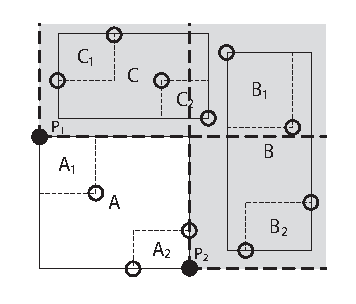
\includegraphics[width=1.5in]{Figures/index_based_pruning_b.eps}
    %\end{minipage}
    }
  \caption{Index-Based Pruning Strategies (min, min)}
  \label{fig:ibp}
\end{figure}

IPS is shown in Algorithm~\ref{alg:IBSkyline}. The initialization and outer loop is the same as RPS. During skyline computation phase (line 13-30), the next expected item (index or data bucket) is popped from the stack and downloaded from the channel. If the item is an index, then each inner (bounding box, broadcast time) pair is checked to see if $R$ covers the bounding box (line 9). If the bounding box is not covered, then the pair is pushed onto the stack, and $n$ pruning regions are computed as follows:

\begin{enumerate}
\item The next level bounding box is pushed onto the stack to be downloaded in future iteration (line 20).
\item The local pruning region, $R'$ is computed from the next level bounding box (line 21).
\item Candidate skyline and queue entries that are covered by $R'$ are removed (line 22-23).
\item Local pruning regions, $R'$, is added to the global pruning regions (line 24).
\end{enumerate}

If the downloaded item is a data bucket, then skyline is computed from the bucket and added to the set of candidate skyline (line 28). As in RPS, when the stack is empty, $S$ is returned as skyline result.

\begin{algorithm}
\algsetup{linenosize=\small,linenodelimiter=. }
\caption{Index-Based Skyline($\sigma$)} \label{alg:IBSkyline}
\begin{algorithmic}[1]

\STATE $S$ $\gets$ $\emptyset$
\STATE $R$ $\gets$ $\emptyset$
\REPEAT
    \STATE next $\gets$ null

    \IF {first iteration}
        \STATE bucket $\gets$ search first index bucket
    \ELSE
        \STATE bucket $\gets$ GetBucket(next)
    \ENDIF

    \IF {!IsRootNode(bucket)}
        \STATE next $\gets$ bucket.time\_of\_next\_index\_segment
    \ENDIF

    \WHILE{!stack.IsEmpty || first iteration}
        \IF {not first iteration}
            \STATE bucket $\gets$ GetBucket(stack.pop)
        \ENDIF
        \IF {IsIndex(bucket)}
            \FOR {$E_i$ in index, $i$ = $b$ to 1}
                \IF {!Covers(R, $E_i$)}
                    \STATE stack.push($E_i$)
                    \STATE $R'$ $\gets$ GetPRegions(e.mbr, $\sigma$)
                    \STATE Prune($S$, $R'$)
                    \STATE Prune(stack, $R'$)
                    \STATE $R$ $\gets$ $R$ $\cup$ $R'$
                \ENDIF
            \ENDFOR
        \ELSE
            \STATE $S$ $\gets$ $S$ $\cup$ Skyline(bucket, $\sigma$)
        \ENDIF
    \ENDWHILE
\UNTIL {next = 0}
\RETURN $S$
\end{algorithmic}
\end{algorithm}

%\begin{algorithm}
%\algsetup{linenosize=\small,linenodelimiter=. }
%\caption{ComputePruneRegion($S$, $\sigma$)}
%\label{alg:ComputePruneRegion1}
%\begin{algorithmic}[1]
%
%\STATE $totalR \gets$ \o \FORALL{$p$ in $S$}
%    \STATE $tempR \gets$ ($-\infty$ to $\infty$) for all dimensions
%    \FOR{$i = 0$ to $n$}
%        \IF{$\sigma[i] = MIN$}
%            \STATE $tempR \gets tempR \bigcap (\infty \bigcup ... \bigcup (s[i]~to~\infty)_i \bigcup ... \bigcup \infty $)
%        \ELSE
%            \STATE $tempR \gets tempR \bigcap (\infty \bigcup ... \bigcup (min(D_i)~to~s[i])_i \bigcup ... \bigcup \infty $)
%        \ENDIF
%    \ENDFOR
%    \STATE $totalR \gets totalR \bigcup tempR$
%\ENDFOR \RETURN $totalR$
%\end{algorithmic}
%\end{algorithm}


%\begin{algorithm}
%\algsetup{linenosize=\small,linenodelimiter=. }
%\caption{ComputePruneRegion($B$, $\sigma$)}
%\label{alg:ComputePruneRegion2}
%\begin{algorithmic}[1]
%\STATE $R \gets$ \o \FOR{$i = 0$ to $n$}
%    \IF{$\sigma[i] = MIN$}
%        \STATE Add dimension $i$ to $R$ from 0 to $\infty$
%    \ELSE
%        \STATE Add dimension $i$ to $R$ from 0 to $B.i_{max}$
%    \ENDIF
%\ENDFOR \RETURN $R$
%\end{algorithmic}
%\end{algorithm}

%\subsubsection{Data Preparation}
%The data and index preparation is the same as in Solution1. The only difference is that instead
%of indexing the data with R-Tree, this solution index the data with R+-Tree. The attractiveness of
%this index structure is non-overlapping MBR and we can quickly find the pruning region in our
%algorithm. Give an example of why overlapping would cause a problem.

%A drawback of this index technique is creating an R-Tree without overlapping MBRs incur
%computational overhead (cite).


%\subsubsection{Skyline Computation}
%
%We start with pruning region that covers space. As soon as our algorithm receives the first index
%segment we get a sense of the data distribution in space we can start forming pruning regions.
%Consider example [provide example and attach figure].  The entire index tree consists of MBRs
%A and B. Let $Min(MBR)$ be the corner of MBR that has minimum of all dimension and $Max(MBR)$
%be the corner that has maximum of all dimension. Since $Min(B)$ < $Min(A)$, we can immediately
%form the pruning region, and prune MBR A.

%Note, we don't need to consider sub-MBRs inside A and B. Since the MBRs do not overlap, the
%entire region cover by A is dominated by B. Comparing with Solution 1, we don't have to traverse
%the tree to the leaf nodes to start forming pruning regions; instead, we can obtain pruning regions
%as early as the root node of the index. This has improvement in tuning time.


%\subsubsection{Correctness Verification}

%We consider the correctness of this algorithm for the MIN $x$, MIN
%$y$ case. This verification can be easily applied to other cases
%with combinations of attribute specifiers. Our goal is to prove
%the correctness of our index-based pruning algorithm. We want to
%show that we can form pruning regions from the MBR of an index
%node instead of wait until we receive data records as in
%Algorithm~\ref{alg:PBSkyline}. We also want to show that this
%algorithm does not prune false negatives (more than it should
%prune).
%
%We can form pruning region from the MBR of the index because the
%MBR of R+-Tree does not overlap. As we mentioned earlier in this
%paper, this technique does not work for index structures that
%allow overlapping index regions such as R-Tree and R*-Tree
%\cite{Beckmann:1990:RER:93597.98741}.
%
%Given a MBR, $b$, of data index that encloses data records, the
%$b$ is bounded by two points $(x_{min}, y_{min})$, $(x_{max},
%y_{max})$ and these points denote the lower-left and upper-right
%corners of the MBR respectively. There must exist a point, $p_1$,
%in $b$ such that $p_1.y = b.y_{min}$, $p_1.x$ in range
%$[b.x_{min}, b.x_{max}]$. Similarly, there must exist another
%point, $p_2$ such that $p_2.x = b.x_{min}$, $p_2.y$ in range
%$[b.y_{min}, b.y_{max}]$.
%
%$p_1$ dominates anything to the right of $p_1.x$ and above
%$b.y_{min}$ and $p_2$ dominates all records above $p_2.y$ and to
%the right of $b.x_{min}$. We extend the $y$ value of the prune
%region of $p_1$ and the $x$ value of the pruning region of $p_2$
%and these two are the same as the values for the pruning region of
%point $(b.x_{min}, b.y_{min})$. Since MBRs do not overlap, pruning
%regions for point $(b.x_{min}, b.y_{min})$ is the pruning region
%of the MBR $b$.

%\subsection{Skyline of Higher-Dimension}
%For skyline queries that involves more than two query attributes,
%we need to consider computation of skyline of higher dimension.
%Due to the generic nature of our algorithm, we can extend our
%algorithm to higher dimensions.
%
%Similar to skyline in two-dimension, we first need to index our
%data in an index structure. R-Tree and other spatial index
%structure, such as KD-Tree, can support data of arbitrary
%dimension. KD-Tree and Quad-Tree are better choice here due to
%lower computation complexity of building the index for
%higher-dimensional data. %We build our index as illustrated in Figure \ref{fig:rtree3d}.

%\begin{figure}[h]
%\begin{center}
%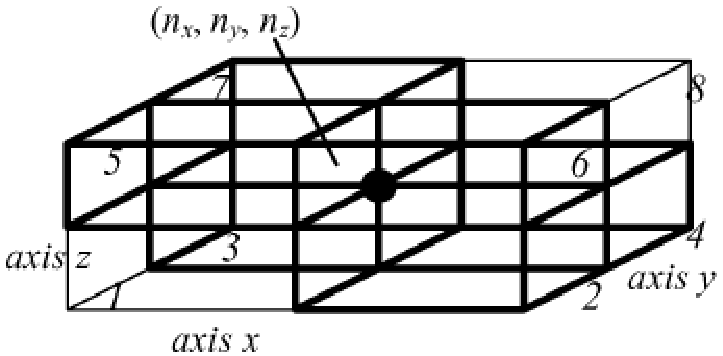
\includegraphics[width=3in]{Figures/rtree3d-eps-converted-to.pdf}
%\caption{\small Data Records inserted into R-Tree.\label{fig:rtree3d}}
%\end{center}
%\end{figure}

%Using the index, we can compute higher-dimensional pruning region
%(space) to facilitate skyline computation.

\subsection{Analysis}

In this section we consider tuning time and access latency of the
two pruning region skyline algorithms we presented in this
section. We assume that the client makes skyline queries at the
beginning of a cycle. Since the amount of time spent listening to
the channel is the amount of time required for a client to get all
the desired data, the tuning time is equal to access latency;
therefore, we use the same analysis for both quantities.

We first consider the tuning time for the algorithm that uses the
record-based pruning strategy. The best case is that the client
gets all desired data from the first data segment, and the rest of
the cycle is pruned. In this case, $\beta = h \times \eta +
\varsigma$. The expected case is when the client has to listen to
half of the program and $E(\beta) = \frac{1}{2}(\iota + \theta)$

We now consider the same quantity for the index-based pruning
skyline algorithm. The assumption is the same as before, but a
client does not have to traverse the index to the leaf level
before they start pruning. On average, a client would have to
traverse half of the index tree but would still have to download
half of the data; therefore $E(\beta) = \frac{1}{4}\iota +
\frac{1}{2}\theta$

%\subsubsection{No Index}
%
%When no index is added to the broadcast cycle, the program
%length is equal to the number of data packets. The tuning time, $t_t$
%and access latency, $t_l$, is also equal to program length since a client
%have to listen to the entire broadcast cycle to compute the skyline.
%
%\begin{equation}
%    l_p = t_t = t_l = d
%\end{equation}
%
%The initial index probing time and the index percentage do not apply
%and we set both to 0.
%
%\begin{equation}
%    t_p = p_i = 0
%\end{equation}
%
%\subsubsection{One-time index}
%
%In one-time index, the index packets only appear one time at the
%beginning of the program without replication. Consider every node
%is pack in one index packet. For a full R-Tree
%index, the following defines the relationship:
%
%\begin{eqnarray}
%% \nonumber to remove numbering (before each equation)
%  h &=& \log_{b} n_t - 1 \\
%  n_i &=& \displaystyle\sum\limits_{i=0}^h b^i \\
%  l_p &=& d + n_i
%\end{eqnarray}
%
%The expected tuning time and access latency is the half of the
%broadcast program:
%
%\begin{eqnarray}
%% \nonumber to remove numbering (before each equation)
%  t_t &=& \frac{1}{2} (d + n_i) \nonumber \\
%      &=& \frac{1}{2} (d + \displaystyle\sum\limits_{i=0}^h b^i) \\
%  t_l &=& t_t
%\end{eqnarray}
%
%\subsubsection{DFDI}
%
%Assume r percent of the index is replicated and the rest is not
%replicated, the program length is as follows:
%
%\begin{equation}
%    l_p = d + (1 + r) \displaystyle\sum\limits_{i=0}^h b^i
%\end{equation}
%
%The expected tuning time and access latency is the same as for the
%one-time index that is the half of the length of the broadcast
%program. Note that, even though, the function of these two metrics
%are the same, the program length is different for both cases.
%For DFDI, since we replicated $r$ percent of the index, the program
%length is longer, therefore, the latency and tuning time are also
%longer.

%The formulation of a pruning region depends on a pivot point, here we denote
%it with $p$, and the preference specifiers
%of the attributes of the data. For each axis (attribute) of the data space,
%the preference could be either MIN or MAX. For an axis $i$ with MIN specifier,
%the pruning space is from $p.i$ to $\infty$ (or maximum value for the attribute).
%Similarly, for the axis with MAX specifier, the pruning space is from $p.i$ to
%$-\infty$ or minimum value of the attribute. For data of positive value, the
%minimum value would be 0.
